\documentclass[fleqn]{article}

\usepackage{mydefs}
\usepackage{notes}
\usepackage{url}
\usepackage{graphicx}
\usepackage{textcomp}
\usepackage{amsmath}
\graphicspath{ {./images/} }

\begin{document}
\lecture{Computer Vision}{HW2: Feature Detection and Panoramas}{Dan Engbert, QD36731}
\section{Coding Assignment}
The goal of this assignment is to implement 3 forms of image features to be used for binary classification of images of dogs and cats.

\subsection{Testing Strategy}
I created a function called crossValidation() that combines the training set and validation set, then splits that into k sections.  Then k-fold cross validation is performed; for each fold imdb.test\_indices is set to the indices in that fold, and train\_indices is set to the remaining indices.  Then features are generated and the model is trained and the accuracy of the trial is recorded.  At the end, the average accuracy across all k-trials is computed and can be used as a metric for evaluating the effectiveness of different parameters for the model.  The parameter \textit{--cross}  was added to have the code perform cross validation rather than testing on the test set and to allow the user to specify the number of folds to partition the data into.

Once the optimal parameters are found, the code is run again (without the \textit{--cross} flag) but this time the model is trained using the entire (original) train+val data set, and then evaluated on the test set. 

\section{Feature Techniques}



\subsection{tinyimage}
The first feature implemented was tinyimages.  This method creates a feature vector for each image by scaling it down to a fixed [n n 3] (3 color channel image with dimensions nxn) and then flattening it into a vector of size [1 nxnx3].

\subsubsection{KNN Results}
I used 5-fold cross validation, and kept tweaking one parameter at a time to see how the average accuracy from the cross validation changed.  The average accuracy over 5-folds with these parameters tended to be the highest (ranging from 62\% to 69\%) compared to other parameters.

Best results using KNN with these features (with 5-fold cross validation) were obtained with the parameters:
\begin{solution}
./main.py -d ../data/ -f tinyimage --tinyimage-patchdim 7  -c knn -k 5
\end{solution}

Confusion Matrix (trainining set: train+val, test set: test):
\[
  \begin{bmatrix}
    40 & 10 \\
    29 & 21
  \end{bmatrix}
\]
This is an overall accuracy of 61.0\%.

So the performance on the test set was not quite as good as with the cross-validation.
\begin{center}
    \makebox[\textwidth]{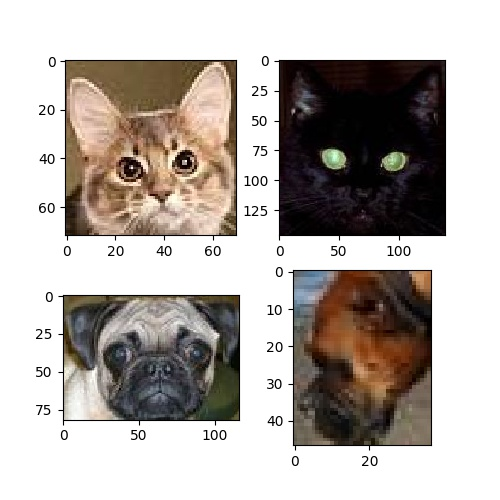
\includegraphics[width=0.3\paperwidth]{tiny_knn_confusion.jpg}}
    Most Cat-Like Cat (top left), Most Dog-Like Cat (top right)\break
    Most Cat-Like Dog (bottom left), Most Dog-Like Dog (bottom right)
\end{center}

\subsubsection{SVM Results}
Again I used 5-fold cross validation, and kept tweaking one parameter at a time to see how the average accuracy from the cross validation changed.  The best parameters are show below:
\begin{solution}
    ./main.py -d ../data/ -f tinyimage --tinyimage-patchdim 6 -c svm -l 1.0
\end{solution}
The average accuracy over 5-folds with these parameters tended to be the highest (ranging from 64\% to 69\%) compared to other parameters.

Results when the above parameters were applied to the test set:

Confusion Matrix (trainining set: train+val, test set: test):
\[
  \begin{bmatrix}
    32 & 18 \\
    19 & 31
  \end{bmatrix}
\]
This is an overall accuracy of 63.0\%.
\begin{center}
    \makebox[\textwidth]{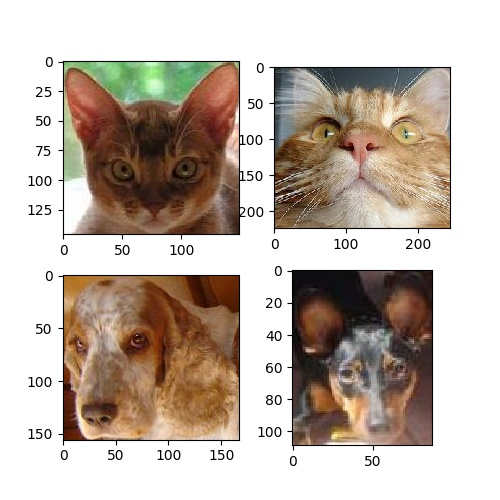
\includegraphics[width=0.3\paperwidth]{tiny_svm_confusion.jpg}}
    Most Cat-Like Cat (top left), Most Dog-Like Cat (top right)\break
    Most Cat-Like Dog (bottom left), Most Dog-Like Dog (bottom right)
\end{center}



\subsection{bow-patches}
Bow-patches works by sampling small squares of (grayscale) pixels across images in the training set, then flattening each patch into a vector.  After a sufficient number of patches have been sampled (100 times the dictionary size), they are clustered using k-means and the cluster centers are then used as the dictionary "bag of words."  Then all training images are broken into patches and each patch is matched with the closest word in the dictionary (the vector with the lowest euclidean distance).  A histogram counting the "visual words" within each image is then generated and normalized by dividing each element of the feature by the sum of the feature.  The features are then used to train a model (either a KNN model or SVM).

\subsubsection{KNN Results}
I wrote a script that tried over 90 different combinations of parameters using 3-fold cross validation and the best result had an average validation accuracy of 61\%.  When manually tweaking the dictionary size afterwards (using the best parameters found by the script), I found that results started to get noticably worse (55\% to 58\% accuracy) when the dictionary size was 90 or less.  I also tested with a dictionary size of 200, and the cross-validation average accuracy was 58\% which is not noticably better than with a dictionary of size 128.
\begin{solution}
    ./main.py -d ../data/ -f bow-patches --patches-dictionarysize 128 --patches-radius 8 --patches-stride 11  -c knn -k 7
\end{solution}
Results when the above parameters were applied to the test set:

Confusion Matrix (trainining set: train+val, test set: test):
\[
  \begin{bmatrix}
    25 & 25 \\
    12 & 38
  \end{bmatrix}
\]
This is an overall accuracy of 63.0\%.
\begin{center}
    \makebox[\textwidth]{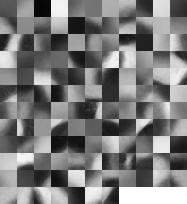
\includegraphics[width=0.2\paperwidth]{patch_knn_dictionary.jpg}}
    Visualized Dictionary
\end{center}
\begin{center}
    \makebox[\textwidth]{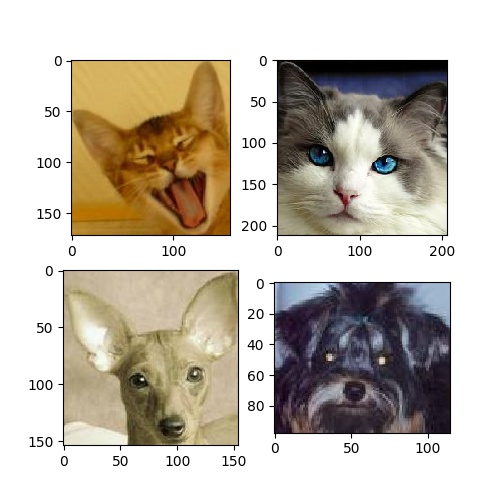
\includegraphics[width=0.3\paperwidth]{patch_knn_confusion.jpg}}
    Most Cat-Like Cat (top left), Most Dog-Like Cat (top right)\break
    Most Cat-Like Dog (bottom left), Most Dog-Like Dog (bottom right)
\end{center}

\subsubsection{SVM Results}
I performed 3-fold cross validation to test varying parameters for building an SVM model.  I started with the same dictionary size, radius, and stride used with KNN, then slowly adjusted them to attempt to maximize the average (cross validation) lableing accuracy.  I found that a dictionary size of 60 was effective and a radius of 10, stride 4, and lamda 110.  Increasing or decreasing the dictionary size (from 60) did not lead to any impovements, and the same held for the radius, stride, and lambda.  To account for the small dictionary size, I allowed the set of patches trained on to be 310 times the size of the dictionary (rather than 110 as I did previously when using a dictionary size of 128).  Dictionary sizes of 30 and 90 were also tested but showed no improvment.
\begin{solution}
    ./main.py -d ../data/ -f bow-patches --patches-dictionarysize 60 --patches-radius 10 --patches-stride 6  -c svm -l 110
\end{solution}
Results when the above parameters were applied to the test set:

Confusion Matrix (trainining set: train+val, test set: test):
\[
  \begin{bmatrix}
    37 & 13 \\
    22 & 28
  \end{bmatrix}
\]
This is an overall accuracy of 65.0\%.
\begin{center}
    \makebox[\textwidth]{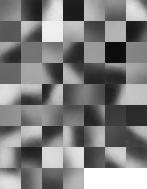
\includegraphics[width=0.2\paperwidth]{patch_svm_dictionary.jpg}}
    Visualized Dictionary
\end{center}
\begin{center}
    \makebox[\textwidth]{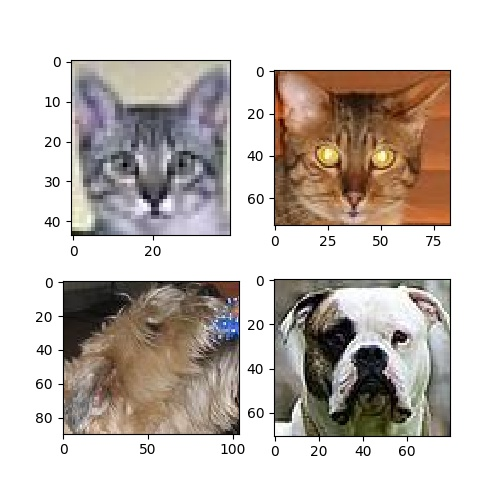
\includegraphics[width=0.3\paperwidth]{patch_svm_confusion.jpg}}
    Most Cat-Like Cat (top left), Most Dog-Like Cat (top right)\break
    Most Cat-Like Dog (bottom left), Most Dog-Like Dog (bottom right)
\end{center}




\subsection{bow-sift}
Bow-sift works the same as bow-patches, except that rather than flattening each patch into a vector to use as a feature, a SIFT descriptor is computed for the center pixel of that patch.  The computed SIFT descriptor is then used as the feature vector.
\subsubsection{KNN Results}
I played around with adjusting the parameters and the best results while doing 3-fold cross validation were with the following parameters:
\begin{solution}
    ./main.py -d ../data/ -f bow-sift --sift-dictionarysize 128 --sift-binsize 15 --sift-radius 8 --sift-stride 12 -c knn -k 4
\end{solution}
Results when the above parameters were applied to the test set:

Confusion Matrix (trainining set: train+val, test set: test):
\[
  \begin{bmatrix}
    36 & 14 \\
    19 & 31
  \end{bmatrix}
\]
This is an overall accuracy of 67.0\%.
\begin{center}
    \makebox[\textwidth]{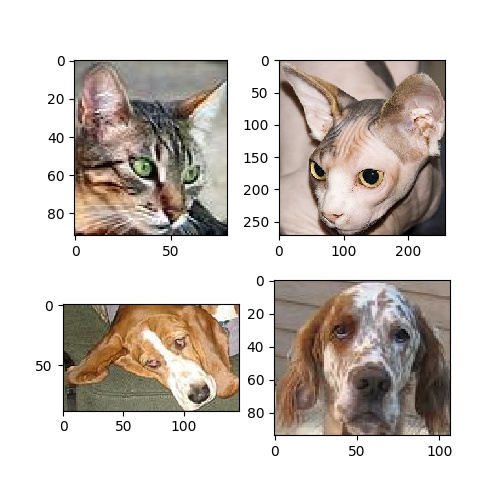
\includegraphics[width=0.3\paperwidth]{sift_knn_confusion.jpg}}
    Most Cat-Like Cat (top left), Most Dog-Like Cat (top right)\break
    Most Cat-Like Dog (bottom left), Most Dog-Like Dog (bottom right)
\end{center}

\subsubsection{SVM Results}
I performed 3-fold cross validation using SVM to build the model.  I found that the dictionary size wasn't too important, it just needed to be roughly between 100 and 200.  Values of 128 and 200 led to similar results (about 69\% detection accuracy).  As with bow-patches, I found that larger values of lamda (between 100 and 150) worked the best (small values such as 1.0 led to horrible results).  I found that a radius around 8 or 9 and a stide between 6 and 12 was effective and adjusting the bin size between 5 and 10 did not have too much of an effect.  The best combinations of parameters led to cross-validation accuracy results between 68\% and 71\%.

The best results in cross-validation were obtained with the following parameters:
\begin{solution}
    ./main.py -d ../data/ -f bow-sift --sift-dictionarysize 150 --sift-binsize 10 --sift-radius 9 --sift-stride 6 -c svm -l 115
\end{solution}
Results when the above parameters were applied to the test set:

Confusion Matrix (trainining set: train+val, test set: test):
\[
  \begin{bmatrix}
    45 & 5 \\
    16 & 34
  \end{bmatrix}
\]
This is an overall accuracy of 79.0\%.

These parameters happened to lead to better performance on the test set than in cross-validation testing (where the average accuracy was 71.5\%).
\begin{center}
    \makebox[\textwidth]{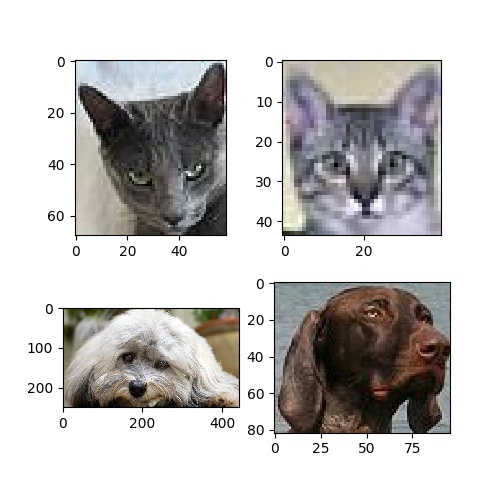
\includegraphics[width=0.3\paperwidth]{sift_svm_confusion.jpg}}
    Most Cat-Like Cat (top left), Most Dog-Like Cat (top right)\break
    Most Cat-Like Dog (bottom left), Most Dog-Like Dog (bottom right)
\end{center}



\section{Discussion}
I found that SVM consistently performed slightly better than KNN across all 3 features.  To achieve the best results with each feature, quite different parameters had to be used (the optimal dictionary size and radius/stride varied when using SVM vs KNN on bow-patches and bow-stride.

While testing with cross-validation, the accuracy between KNN and SVM with the tiny-image features was the closest compared to with the other two features.  I would possibly attribute this to the fact that color was kept in the tiny images prior to flattening them to a vector.  When you shrink the images to a really small size (like 7x7 pixels), the color will play an important part in the vector.  Perhaps cat images tend to be brighter colors and the dogs tend to be darker; this would help KNN because the cats would be closer to each other in the vector space.
\end{document}
